% CVPR 2025 Paper Template; see https://github.com/cvpr-org/author-kit
\documentclass[10pt,twocolumn,letterpaper]{article}
\usepackage{amsmath}
\usepackage{amssymb}
\usepackage{amsthm}
\usepackage{authblk}
\usepackage{latexsym}
\usepackage{array}
\usepackage{booktabs}
\usepackage{multirow}
\usepackage{makecell}
\usepackage{graphicx}
\usepackage{stfloats}
\usepackage[shortlabels, inline]{enumitem}
\usepackage{appendix}
\usepackage{color}
\usepackage[hyphens]{url}
\usepackage[ruled,linesnumbered]{algorithm2e}
\usepackage{cvpr}
\usepackage[pagebackref,breaklinks,colorlinks,allcolors=cvprblue]{hyperref}

% 颜色定义
\definecolor{cvprblue}{rgb}{0.21,0.49,0.74}

% 定理环境定义
\newtheorem{corollary}{Corollary}
\newtheorem{theorem}{Theorem}
\newtheorem{definition}{Definition}
\newtheorem{problem}{Problem}
\newtheorem{assumption}{Assumption}

% Autoref 定制
\DeclareRobustCommand{\corollaryautorefname}{Corollary}
\DeclareRobustCommand{\problemautorefname}{Problem}
\DeclareRobustCommand{\theoremautorefname}{Theorem}
\DeclareRobustCommand{\assumptionautorefname}{Assumption}

% 其他配置
\newcommand{\CG}{\mathcal{G}\xspace}
\newcommand{\CV}{\mathcal{V}\xspace}
\newcommand{\CE}{\mathcal{E}\xspace}
\newcommand{\CA}{\mathcal{A}\xspace}
\newcommand{\CF}{\mathcal{F}\xspace}
\newcommand{\CR}{\mathcal{R}\xspace}
\newcommand{\CB}{\mathcal{B}\xspace}
\newcommand{\CX}{\mathcal{X}\xspace}
\newcommand{\CK}{\mathcal{K}\xspace}
\newcommand{\CM}{\mathcal{M}\xspace}
\newcommand{\CC}{\mathcal{C}\xspace}
\newcommand{\CL}{\mathcal{L}\xspace}
\newcommand{\CI}{\mathcal{I}\xspace}
\newcommand{\CQ}{\mathcal{Q}\xspace}
\newcommand{\CO}{\mathcal{O}\xspace}
\newcommand{\CP}{\mathcal{P}\xspace}
\newcommand{\CS}{\mathcal{S}\xspace}
\newcommand{\CT}{\mathcal{T}\xspace}
\newcommand{\CJ}{\mathcal{J}\xspace}
\usepackage[para]{footmisc}
\usepackage{subfig}
% \usepackage{subcaption}
% \usepackage{array}
% \usepackage{colortbl}



\def\paperID{342} 
\def\confName{CVPR}
\def\confYear{2025}

\title{Order-Robust Class Incremental Learning: Graph-Driven \\ Dynamic Similarity Grouping}
\author[1]{Guannan Lai$^{\dag}$}
\author[1, 2]{Yujie Li$^{\dag}$}
\author[1]{Xiangkun Wang}
\author[3]{Junbo Zhang}
\author[4]{Tianrui Li}
\author[1]{Xin Yang$^{\star}$}
\affil[1]{School of Computing and Artificial Intelligence, Southwestern University of Finance and Economics, 
\authorcr \textit{Email: aignlai@163.com, \{liyj1201, xiangkunwang18\}@gmail.com, yangxin@swufe.edu.cn}}

\affil[2]{LIACS, Leiden University,}

\affil[3]{JD Intelligent Cities Research, \textit{Email: msjunbozhang@outlook.com}}

\affil[4]{Southwest Jiaotong University, \textit{Email: trili@swjtu.edu.cn}}


\begin{document}
\maketitle

\footnotetext[1]{$^{\dag}$ Equal contribution, sorted alphabetically.}
\footnotetext[2]{$^{\star}$ Corresponding author.}

\input{arxiv_sections/0}
\section{Introduction}
Class Incremental Learning (CIL) necessitates that the model dynamically acquires knowledge of new classes while preserving the knowledge of previously learned classes within an infinite sequence of tasks \cite{wang2019forward,ke2021achieving,NEURIPS2023_15294ba2}. 
CIL is realistic but a great challenge for deep neural networks \cite{parisi2019continual}, where existing works devoted to overcoming catastrophic forgetting (CF) and encouraging knowledge transfer across different tasks \cite{mccloskey1989catastrophic,ye2020heterogeneous,zhao2021mgsvf,wang2024comprehensive}.
With the rapid advancement of CIL, a growing number of methods \cite{yoon2019scalable,li2024hessian,shan2024order} have been introduced to address the problem of CF from the perspective of the order in which classes appear (or task order).
In practice, the arrival order of each class and the tasks to which they belong are random and the order in which tasks arrive is uncontrollable \cite{bell2022effect}, further resulting in \textit{Class order sensitivity} and \textit{Intra-task class conflicts} \cite{lin2023theory}. 
Therefore, designing an order-robust CIL method is essential for the community.

\begin{figure}[t]
    \centering
    \includegraphics[width=1\linewidth]{figures/1.pdf}
    \caption{The crucial challenges of CIL (illustration on CIFAR100 dataset). On the left subfigure (a), each model’s performance is shown under varying class orders, testing its robustness to class order sensitivity. On the right subfigure (b), the model’s performance is shown when classes within the same task are similar, evaluating its resilience to intra-task classes with high similarities.}
    \label{fig: intro}
\end{figure}

\textit{Class order sensitivity} refers to the model exhibiting significant performance variations depending on the sequence in which classes are introduced \cite{shan2024order}. 
This phenomenon is prevalent in real-world applications (see \autoref{fig: intro}(a)). 
For instance, in online recommendation systems, the order in which user data classes are received at different time points is difficult to control. If the system initially receives data from relatively few classes, the introduction of subsequent classes may impair the system’s adaptability, resulting in unstable model performance on new tasks.
Furthermore, the model’s parameters may be overfitted to the classes of early tasks, diminishing its ability to generalize to subsequent task with new classes.
Although existing research, such as APD \cite{yoon2019scalable} and HALRP \cite{li2024hessian}, have attempted to mitigate the class order sensitivity problem by modifying network structures, their effectiveness remains limited and has not fundamentally addressed this challenge. 
Thus, designing a model capable of maintaining stable performance across varying class orders remains a critical unsolved issue in CIL.

\textit{Intra-task class conflicts} refers to the discrepancies in model performance caused by the similarity between classes that are trained simultaneously in a specific task (see \autoref{fig: intro}(b)). 
In real-world applications, where the arrival of classes in the data stream is uncontrollable, significant similarities among classes can severely impact the model's resilience. 
For example, in a specific task from a sequence of tasks, a model may be trained to recognize different breeds within the same species. Within this task, due to the high similarity of features across categories, the model needs to develop resilience in distinguishing between closely related classes.
However, existing CIL methods struggle to address this challenge, primarily due to the inherent limitations of the task setting. As CIL incrementally processes different classes, it cannot globally account for all class information, causing class conflicts to accumulate during training and negatively impact model performance. Thus, alleviating class conflicts and improving the model’s generalization ability remains a significant challenge in CIL.

Hence, to tackle the challenges of class order sensitivity and Intra-task class similarity sensitivity, we first conduct an in-depth analysis beyond existing theories. 
Our theoretical findings suggest that as class similarity decreases in CIL, the model's robustness to class order increases, which, in turn, mitigates knowledge conflicts both across different tasks and within individual tasks.
Then, we propose a similarity graph-based dynamic grouping method, called \textbf{Graph-Driven Dynamic Similarity Grouping (GDDSG)}, to maintain the centroids of existing classes and dynamically groups tasks based on class similarity, assigning classes with lower similarity to the same group.
This approach innovatively organizes class groups in CIL by utilizing a graph-based technique to minimize inter-group similarity. It dynamically assigns classes based on adaptive similarity thresholds and optimal graph coloring, thereby enhancing model robustness and computational efficiency across tasks.
In the incremental learning process, GDDSG continuously updates existing groups or creates new ones, training a separate model for each group. Consequently, during the prediction phase, decisions are made by aggregating the outputs of multiple models.

Hence, our contributions can be summarised as follows:
\begin{itemize}
    \item In this paper, we elaborate on existing theories and derive an important Corollary: when the similarity between classes is low, the model's sensitivity to class order is significantly reduced, leading to a decrease in class conflicts.

    \item Then, we provide a detailed introduction to the proposed GDDSG method, including its foundational algorithms and basic processes.

    \item Additionally, we conduct extensive comparative experiments to validate the effectiveness of GDDSG, highlighting its advantages and potential in incremental learning tasks.
\end{itemize}
\section{Background}

\subsection{Multi-Agent Deep Reinforcement Learning}
 A typical system consists of the following components: agents, an environment, and a training algorithm, as depicted in Figure~\ref{fig:madrl_system}. Formally, we consider a system with $N$ agents, each indexed by $i \in \{1, \dots, N\}$. At each time step, the agent $i$ is presented with an observation $o_i$ and produces an action $a_i$. For the sake of generality, we included a possible communication channel $c_i$, seeing that it is increasingly used \cite{Zhu2022ASO}. In principle, we can extend the definition of communication to include the most common MADRL methods like parameter sharing \cite{Gupta2017CooperativeMC,Chu2017ParameterSD}, which can be seen as a form of latent space communication. Finally, the training algorithm provides feedback $\nabla_i$ to each agent.

Training algorithms in MADRL can be centralized, decentralized, or hybrid. Centralized training uses the joint action $a=(a_1,...,a_N)$ and the state $s$, which can be understood as an observation augmented by information at training time \cite{Lambrechts2023InformedPL}, and consists of applying classical RL to multi-agent problems like for AplhaStar \cite{Mathieu2023AlphaStarUL}. While decentralized training restricts each agent to local observations $o_i$, possibly including a local reward $r_i$, see IDQN \cite{Tampuu2015MultiagentCA} or IPPO \cite{Yu2021TheSE}. Hybrid approaches, such as centralized training with decentralized execution, leverage global information during training but allow agents to act independently using only local observations during execution, see VDN \cite{Sunehag2017ValueDecompositionNF}, QMIX \cite{Rashid2018QMIXMV}, MADPG \cite{Lowe2017MultiAgentAF} or MAPPO \cite{Yu2021TheSE}. Here, we consider agents based on DNNs; therefore, the feedbacks $\nabla_i$ are gradients of a loss $\ell$. Depending on the training algorithm, this loss can be a function of the reward $r$, the state $s$, the actions $a_i$, the observations $o_i$ and the communications $c_i$. For simplicity, we didn't include those dependencies in Figure~\ref{fig:madrl_system}.
 
\begin{figure}[ht]
    \centering
    \includegraphics[width=\linewidth]{figures/MADRL.pdf}
    \caption{Schema of a simplified view of MADRL systems. At each time step, the agent $i$ receives the initial observation $o_i$, complemented by potential communications $c_i$ and produces an action $a_i$. The agent learns throughout training by the means of gradients $\nabla_i$. }
    \label{fig:madrl_system}
\end{figure}


\subsection{Direct Interpretability of DNNs}
\label{sec:background_interp}

We now present an overview of the modern methods widely used to interpret DNNs in Computer Vision (CV) and Natural Language Processing (NLP). As these domains heavily relied on pre-trained models \cite{Simonyan2014VeryDC,He2015DeepRL, Radford2018ImprovingLU}, direct post-hoc methods have dominated the research landscape, providing key hindsight without altering models' architectures.


\paragraph{Feature importance.} Typical methods used in CV to understand convolutional networks involve visualising important pixels, i.e. saliency maps, \cite{Zeiler2013VisualizingAU,Selvaraju2016GradCAMVE}. Other methods compute importance by perturbing the input \cite{Covert2020ExplainingBR}, using the gradients \cite{Radford2015UnsupervisedRL,Selvaraju2016GradCAMVE,Shrikumar2016NotJA, Smilkov2017SmoothGradRN} or locally decomposing relevance \cite{Montavon2015ExplainingNC,Bach2015OnPE}. Recent works in NLP focus on the Transformer architecture and its attention mechanism \cite{Vaswani2017AttentionIA}, providing token-level insights \cite{Wiegreffe2019AttentionIN,Achtibat2024AttnLRPAL}. 


\paragraph{Prototypes:} a class of methods that creates explanations based on characteristic samples. In CV, it is common to analyse neurons using activation maximisation to create pre-images \cite{Mahendran2015VisualizingDC}, or find related images \cite{Chen2020ConceptWF}. Prototypes can be of various forms like perturbed images \cite{Ribeiro2018AnchorsHM}, cropped images \cite{Dreyer2023UnderstandingT} or latent space vector \cite{alain2018understanding,kim2018interpretability}. Recent works based on sparse autoencoders were able to elicit interpretable features in LLMs, i.e., prototypes \cite{Cunningham2023SparseAF}.

\paragraph{Latent manipulation:} techniques that further extend the interpretability of concepts and features by exploring the internal representations learned by models. These methods were introduced in CV with \cite{kim2018interpretability}, later derived as the field of representation engineering \cite{zou2023representation}. Such latent features enable locating, editing, erasing or decoding models' knowledge \cite{Meng2022LocatingAE,belrose2023leace, Ghandeharioun2024PatchscopesAU}, but causally modify or analyse the produced outputs \cite{rimsky2023steering, Kramar2024AtPAE}.

\paragraph{Circuit analysis:} provides a more granular understanding of model internals by examining pathways and dependencies between models' components, usually neurons or attention heads. Circuits were first discovered in CNNs \cite{Olah2020ZoomIA} before being formalised for Transformers \cite{elhage2021mathematical}.  These circuits revealed peculiar models' components that learned precise mechanisms like induction \cite{Olsson2022IncontextLA}. Using specific datasets, relevant circuits can be automatically discovered \cite{conmy2023automated}. More recent works focus on larger models' components at the layer scale \cite{Dunefsky2024TranscodersFI}.


% \begin{table}[H]
%  \begin{center}
%    % \tabcolsep = 2\tabcolsep
%    \begin{tabular}{ll}
%    \toprule
%    \textbf{Methodology} & \textbf{Related Works} \\
%    \midrule
%    Feature Importance & \cite{Zeiler2013VisualizingAU,Selvaraju2016GradCAMVE, Lundberg2017AUA, Bach2015OnPE,Radford2015UnsupervisedRL, Covert2020ExplainingBR, Montavon2015ExplainingNC, Achtibat2024AttnLRPAL, Smilkov2017SmoothGradRN, Wiegreffe2019AttentionIN} \\
%    %Ribeiro2016WhySI
%    %Katz2024BackwardLP
%    Prototypes   & \cite{Ribeiro2018AnchorsHM,Achtibat2022FromAM, Chen2020ConceptWF, Mahendran2015VisualizingDC, alain2018understanding,Cunningham2023SparseAF} \\
%    %Dreyer2023FromHT
%    %bills2023language
%    %Dar2022AnalyzingTI
%    Latent Manipulations & \cite{kim2018interpretability,Meng2022LocatingAE,zou2023representation,rimsky2023steering,belrose2023leace,Kramar2024AtPAE,Ghandeharioun2024PatchscopesAU} \\
%    Circuit Analysis          & \cite{Olah2020ZoomIA,elhage2021mathematical,Olsson2022IncontextLA,conmy2023automated, Dunefsky2024TranscodersFI}\\
%    \bottomrule
%    \end{tabular}
% \caption{Categorisation of modern direct interpretability methods drawn from CV and NLP domains.} \label{tab:interp_methods}
%  \end{center}
% \end{table}




\section{\ADDAND: A New Tractable Representation}
\label{sec:ADDAND}

In order to compute the Shannon entropy of a circuit formula $\varphi(X, Y)$, we need to use the probability distribution over the outputs.
Algebraic Decision Diagrams (ADDs) are an influential compact probability representation that can be exponentially smaller than the explicit representation.
Macii and Poncino~\cite{macii1996exact} showed that ADD supports efficient exact computation of entropy.
However, we observed in the experiments that the sizes of ADDs often exponentially explode with large circuit formulas.
We draw inspiration from a Boolean representation known as the Ordered Binary Decision Diagram with conjunctive decomposition (\OBDDAND)~\cite{lai2017new}, which reduces its size through recursive component decomposition and divide-and-conquer strategies. 
This approach enables the representation to be exponentially smaller than the original OBDD.
Accordingly, we propose a probabilistic representation called Algebraic Decision Diagrams with conjunctive decomposition (\ADDAND) and show it supports tractable entropy computation.
\ADDAND is a general form of ADD and is defined as follows:

\begin{definition}\label{ADDAND-definition}
An \ADDAND is a rooted DAG, where each node $u$ is labeled with a symbol $sym(u)$.
If $u$ is a terminal node, $sym(u)$ is a non-negative real weight, also denoted by $\omega(u)$; otherwise, $sym(u)$ is a variable (called \emph{decision} node) or operator $\wedge$ (called \emph{decomposition} node). 
The children of a decision node $u$ are referred to as the \emph{low} child $lo(u)$ and the \emph{high} child $hi(u)$, and connected by dashed lines and solid lines, respectively, corresponding to the cases where $\mathit{var}(u)$ is assigned the value of $\mathit{false}$ and  $\mathit{true}$. 
For a decomposition node, its sub-graphs do not share any variables.
An \ADDAND is imposed with a linear ordering $\prec$ of variables such that given a node $u$ and its non-terminal child $v$, $\mathit{var}(u) \prec \mathit{var}(v) $.


%An \ADDAND is a rooted DAG, where each node $u$ is either terminal or non-terminal.
%Each terminal node $u$ is labeled with a real weight $\omega(u)$ and a set of implied literals $L(u)$.
%Each non-terminal node $u$ is associated with a variable $\mathit{var}(u)$, two children, and a set of implied literals $L(u)$, which satisfies that $\mathit{var}(u)$ does not appear in $L(u)$ and no variable within $L(u)$ appears in any descendant nodes of $u$.
%The children of non-terminal node $u$ are referred to as the \textit{low} child $lo(u)$ and the \textit{high} child $hi(u)$, and connected by dashed lines and solid lines, respectively, corresponding to the cases where $\mathit{var}(u)$ is assigned the value of $\mathit{false}$ and  $\mathit{true}$. 
%An ADD-L is imposed with a linear ordering $\prec$ of variables such that given a node $u$ and its non-terminal child $v$, $\mathit{var}(u) \prec \mathit{var}(v) $.
\end{definition}

Hereafter, we denote the set of variables that appear in the graph rooted at $u$ as $\mathit{Vars}(u)$ and the set of child nodes of $u$ as $Ch(u)$.
We now turn to show that how an \ADDAND defines a probability distribution:
 
\begin{definition}\label{def:ADDAND-weight}
	Let $u$ be an \ADDAND node over a set of variables $Y$ and let $\sigma$ be an assignment over $Y$. 
    The weight of $\sigma$ is defined as follows:
	\begin{equation*}
		   \omega(\sigma,u) =  
		   \begin{cases}  
			   \mathit{\omega}(u) & \text{terminal} \\  
				\prod_{v \in Ch(u)}{\omega(\sigma,v)} & \text{decomposition} \\  
	            \omega(\sigma,lo(u)) & \text{decision and $\sigma \models  \lnot \mathit{var}(u)$}  \\
	            \omega(\sigma,hi(u)) & \text{decision and $\sigma \models  \mathit{var}(u)$}  \\
		   \end{cases}
	\end{equation*}
    The weight of an non-terminal \ADDAND rooted at $u$ is denoted by $\omega(u)$ and defined as $\sum_{\sigma \in 2^{\mathit{Vars}(u)}}\omega(\sigma,u)$.
    The probability of $\sigma$ over $u$ is defined as $p(\sigma, u) = \frac{\omega(\sigma,u)}{\omega(u)}$.
\end{definition}


Figure \ref{fig:ADDAND-Example} depicts an \ADDAND representing the probability distribution of $\varphi_n^{sep}$ in Example \ref{circuit-example} over its outputs wrt $y_1 \prec y_2 \prec \cdots \prec y_{2n}$. The reader can verify that each equivalent ADD wrt $\prec$ has an exponential number of nodes.
In the knowledge compilation field \cite{darwiche2002knowledge,fargier2014knowledge}, we often uses the notion of succinctness to describe the space efficiency of a representation. 
Due to the following observations, we can see that \ADDAND is strictly more succinct than ADD: OBDD and \OBDDAND are subsets of ADD and \ADDAND, respectively, \OBDDAND is strictly more succinct than OBDD ~\cite{lai2017new}; and each \OBDDAND cannot be represented into a non-OBDD ADD.
%We will formally prove this property in the appendix.





\begin{figure}[h]
\vspace{1.5cm} % 在图形上方添加垂直空间
\resizebox{\linewidth}{!} {
\begin{forest}
	for tree={
		if n children=0{circle, draw, inner sep=2pt}{}, % 叶子节点的样式
		if level=1{edge={draw, solid}}{% 如果是根节点的子节点,边为实线
			if n=1{edge={draw, dashed}}{edge={draw, solid}} % 对于其他节点,第一个子节点为虚线,第二个为实线
		}
	}
	[$\wedge$, circle, draw, minimum width=1cm,
	label={[blue,above=0.01cm]above:$\overbrace{(-\frac{3}{4} \cdot \log\frac{3}{4} - \frac{1}{4} \cdot \log\frac{1}{4}) + \cdots + (-\frac{3}{4} \cdot \log\frac{3}{4} - \frac{1}{4} \cdot \log\frac{1}{4})}^{n}$}
	[$y_1$, circle, draw, minimum width=1cm,
	label={[blue,above=0.1cm]above:$-\frac{3}{4} \cdot \log\frac{3}{4} - \frac{1}{4} \cdot \log\frac{1}{4}$},
	name = y1
	[$y_{n+1}$, circle, draw, minimum width=1cm,
	label={[blue,right=0.1cm]right:$0$}
	[$3$, circle, draw, minimum width=1cm,
	label={[blue,below=0.1cm]below:$0$}]
	[$0$, circle, draw, minimum width=1cm,
	label={[blue,below=0.1cm]below:$0$}]
	]
	[$y_{n+1}$, circle, draw, minimum width=1cm,
	label={[blue,right=0.1cm]right:$0$}
	[$0$, circle, draw, minimum width=1cm,
	label={[blue,below=0.1cm]below:$0$}]
	[$1$, circle, draw, minimum width=1cm,
	label={[blue,below=0.1cm]below:$0$}]
	]
	]
	% y_n 节点
	[$y_n$, circle, draw, minimum width=1cm,
	label={[blue,above=0.1cm]above:$-\frac{3}{4} \cdot \log\frac{3}{4} - \frac{1}{4} \cdot \log\frac{1}{4}$}, name = yn
	[$y_{2n}$, circle, draw, minimum width=1cm,
	label={[blue,right=0.1cm]right:$0$}
	[3, circle, draw, minimum width=1cm,
	label={[blue,below=0.1cm]below:$0$}]
	[0, circle, draw, minimum width=1cm,
	label={[blue,below=0.1cm]below:$0$}]
	]
	[$y_{2n}$, circle, draw, minimum width=1cm,
	label={[blue,right=0.1cm]right:$0$}
	[0, circle, draw, minimum width=1cm,
	label={[blue,below=0.1cm]below:$0$}]
	[1, circle, draw, minimum width=1cm,
	label={[blue,below=0.1cm]below:$0$}]
	]
	]
	]
	\begin{tikzpicture}[overlay]
		% 从 y_2 节点的底部到 y_n 节点的顶部绘制一条路径,并在中间添加省略号
		\path (y1.south) -- (yn.north) node[pos=0.5, fill=white] {$\cdots$};
	\end{tikzpicture}
\end{forest}
}




\caption{An \ADDAND representing the probability distribution of $\varphi_n^{sep}$ in Example \ref{circuit-example} over its outputs. 
According to Proposition \ref{prop:Entropy-proposition}, the computed entropy for each node is marked in blue font.
}
\label{fig:ADDAND-Example}
\end{figure}


\subsection{Tractable Computation of Weight and Entropy}
	%\left| \mathit{Sol}(\varphi(Y \mapsto \sigma)) \right| & \text{$u$ is terminal node and $\sigma \models L(u)$} \\ 
	
	The computation of Shannon entropy of \ADDAND depends on the computation of its weight. 
    We first show that for an \ADDAND node $u$, we can compute its weight $\omega(u)$ in polynomial time.
	\begin{proposition}\label{prop:omega-proposition}
		Given a non-terminal node $u$ in \ADDAND, its weight $\mathit{\omega}(u)$ can be recursively computed as follows in polynomial time:
		%$$\mathit{\omega}(u) = 2^{n_0} \cdot \mathit{\omega}(lo(u)) + 2^{n_1} \cdot \mathit{\omega}(hi(u))$$
		\begin{equation*}
			\mathit{\omega}(u) =  
			\begin{cases}  
				\prod_{v \in Ch(u)}{\mathit{\omega}(v)}  & \text{decomposition}   \\
				2^{n_0} \cdot \mathit{\omega}(lo(u)) + 2^{n_1} \cdot \mathit{\omega}(hi(u))  & \text{decision}
				
			\end{cases}
	\end{equation*}
		where $n_0 = |\mathit{Vars}(u)| - |\mathit{Vars}(lo(u))| - 1 $ and $n_1 = |\mathit{Vars}(u)| - |\mathit{Vars}(hi(u))| - 1$. %and $ m = |\mathit{Vars}(u)| - 1 - \sum_{v \in Ch(u)}{ |\mathit{Vars}(v)|}$. 
		%The model counting of the formula represented by $u$ satisfies $CT(u) = \mathit{\omega}(u)$.
		
		\begin{proof}
            The time complexity is immediate by using dynamic programming.
            We prove the equation can compute the weight correctly by induction on the number of variables of the \ADDAND rooted at $u$.
            It is obvious that the weight of a terminal node is the real value labeled. 
            For the case of the $\wedge$ node, since the variables of the child nodes are all disjoint, it can be easily seen from Definition \ref{prop:omega-proposition}.
            Next, we will prove the case of the decision node.
            Assume that when $|\mathit{Vars}(u)| \le n$, this proposition holds. 
            For the case where $|\mathit{Vars}(u)| = n + 1$, we use $Y_0$ and $Y_1$ to denote $\mathit{Vars}(lo(u))$ and $\mathit{Vars}(hi(u))$, and we have $|Y_0| \le n$ and $|Y_1| \le n$.
            Thus, $\mathit{\omega}(lo(u))$ and $\mathit{\omega}(hi(u))$ can be computed correctly.
            According to Definition \ref{def:ADDAND-weight}, $w(u) = \sum_{\sigma \in 2^{\mathit{Vars}(u)}}\omega(\sigma,u)$.
            The assignments over $\mathit{Vars}(u)$ can be divided into two categories: 
            \begin{itemize}
              %\item The assignment $\sigma \not\models L(u)$: $\omega(\sigma, u) = 0$.
              \item The assignment $\sigma \models \lnot \mathit{var}(u)$: 
              It is obvious that $\omega(\sigma, u) = \omega(\sigma_{\downarrow Y_0}, lo(u))$. 
              Each assignment over $Y_0$ can be extended to exactly $2^{n_0}$ different assignments over $\mathit{Vars}(u)$ in this category. Thus, we have the following equation:
              $$\sum_{\sigma \in 2^{\mathit{Vars}(u)} \land \sigma \models \lnot \mathit{var}(u)}\omega(\sigma, u) = 2^{n_0} \cdot \mathit{\omega}(lo(u)).$$
              \item The assignment $\sigma \models \mathit{var}(u)$: This case is similar to the above case.
            \end{itemize}
            To sum up, we can obtain that $\mathit{\omega}(u) = 2^{n_0} \cdot \mathit{\omega}(lo(u)) + 2^{n_1} \cdot \mathit{\omega}(hi(u))$.	
		\end{proof}
		
	\end{proposition}
	
	Now we explain how \ADDAND computes its Shannon entropy in polynomial time.
	\begin{proposition}\label{prop:Entropy-proposition}
		Given an \ADDAND rooted at $u$, its entropy $\mathit{H}(u)$ can be recursively computed in polynomial time as follows:
		\begin{equation*}
		\mathit{H}(u) =  
		\begin{cases}  
			0 & \text{terminal}   \\
			\sum_{v \in Ch(u)}{\mathit{H}(v)}  & \text{decomposition}   \\
			\begin{gathered}
				p_{0} \cdot (\mathit{H}(lo(u)) + n_0)\\
				+ p_{1} \cdot (\mathit{H}(hi(u)) + n_1)\\
				 - p_{0} \cdot \log p_{0} - p_{1} \cdot \log p_{1}
			\end{gathered} & \text{decision}
		
		\end{cases}
		\end{equation*}
		where  $n_0 = |\mathit{Vars}(u)| - |\mathit{Vars}(lo(u))| - 1 $, $n_1 = |\mathit{Vars}(u)| - |\mathit{Vars}(hi(u))| - 1$, $p_{0} = \frac{2^{n_0} \cdot \mathit{\omega}(lo(u))}{\omega(u)}$, and $p_{1} =  \frac{ 2^{n_1} \cdot \mathit{\omega}(hi(u))}{\omega(u)}$.  
       
		
		
		\begin{proof}
        According to Proposition \ref{prop:omega-proposition}, $\omega(u)$ can be computed in polynomial time, and therefore the time complexity in this proposition is obvious. The case of terminal node is obviously correct, the case of decomposition is immediately from the property entropy is additive, and next we show the correctness of the case of decision.

        Let $H_0(u)$ be $-\sum_{\sigma \models \lnot sym(u)} p(u,\sigma) \log p(u, \sigma)$ and $H_1(u)$ be $-\sum_{\sigma \models sym(u)} p(u,\sigma) \log p(u,\sigma)$. Then $H(u) = H_0(u) + H_1(u)$. 
        We use $X$ to denote  $\mathit{Vars}(lo(u))$.
        $H_0(u) = -\sum_{\sigma \models \lnot sym(u)} p_0 \cdot 2^{-n_0} \cdot p(lo(u),\sigma \downarrow X) \cdot \left(\log p_0 - n_0 + \log p(lo(u),\sigma \downarrow X) \right) = p_{0} \cdot \left(-\log p_{0} + n_0 + \mathit{H}(lo(u))\right)$. The case of $H_1$ is dual.
		\end{proof}
		
	\end{proposition}
	
We close this section by explaining why we use the orderedness in the design of \ADDAND.
Actually, Propositions \ref{prop:omega-proposition}--\ref{prop:Entropy-proposition} still hold when we only use the more general read-once property: each variable appears at most once in each path from the root of an \ADDAND to a terminal node.
First, our experimental results indicate that the linear ordering determined by the minfill algorithm in our tool PSE outperforms the dynamic orderings employed in the state-of-the-art model counters, where the former imposes the orderedness and the latter imposes the read-once property.
Second, \ADDAND can provide tractable equivalence checking between probability distributions beyond this study.

\documentclass{standalone}
%\usetikzlibrary{...}
\usepackage{tikz}
\begin{document}
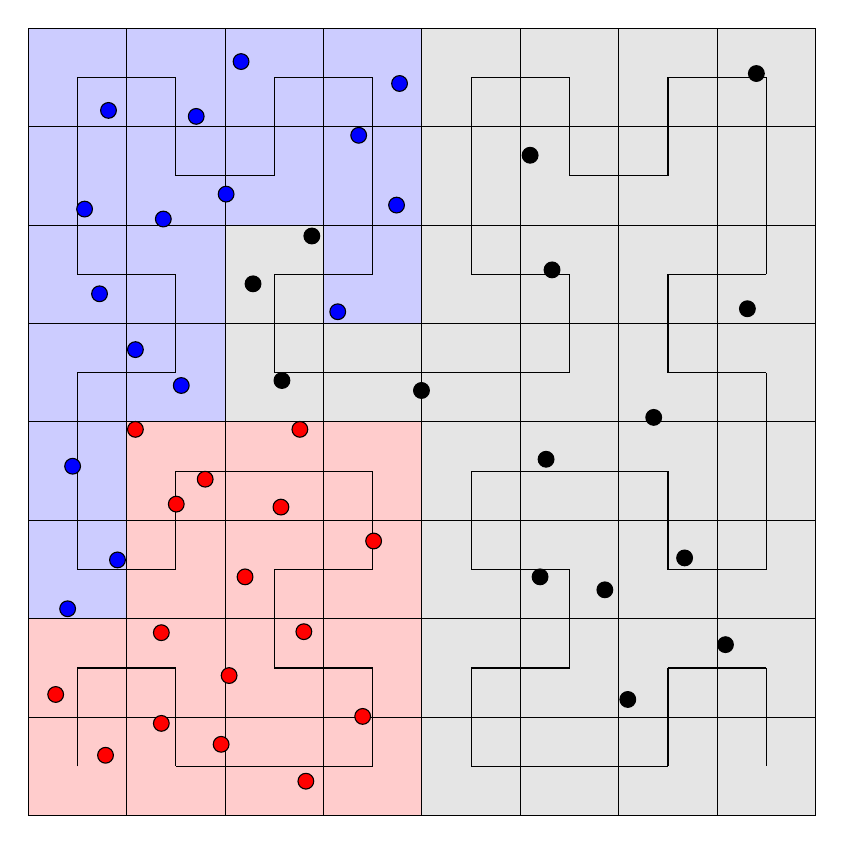
\begin{tikzpicture}
\draw[fill=red!20!white] (0.0, 0.0) rectangle (1.25, 1.25);
\draw[fill=red!20!white] (0.0, 1.25) rectangle (1.25, 2.5);
\draw[fill=red!20!white] (1.25, 1.25) rectangle (2.5, 2.5);
\draw[fill=red!20!white] (1.25, 0.0) rectangle (2.5, 1.25);
\draw[fill=red!20!white] (2.5, 0.0) rectangle (3.75, 1.25);
\draw[fill=red!20!white] (3.75, 0.0) rectangle (5.0, 1.25);
\draw[fill=red!20!white] (3.75, 1.25) rectangle (5.0, 2.5);
\draw[fill=red!20!white] (2.5, 1.25) rectangle (3.75, 2.5);
\draw[fill=red!20!white] (2.5, 2.5) rectangle (3.75, 3.75);
\draw[fill=red!20!white] (3.75, 2.5) rectangle (5.0, 3.75);
\draw[fill=red!20!white] (3.75, 3.75) rectangle (5.0, 5.0);
\draw[fill=red!20!white] (2.5, 3.75) rectangle (3.75, 5.0);
\draw[fill=red!20!white] (1.25, 3.75) rectangle (2.5, 5.0);
\draw[fill=red!20!white] (1.25, 2.5) rectangle (2.5, 3.75);
\draw[fill=blue!20!white] (0.0, 2.5) rectangle (1.25, 3.75);
\draw[fill=blue!20!white] (0.0, 3.75) rectangle (1.25, 5.0);
\draw[fill=blue!20!white] (0.0, 5.0) rectangle (1.25, 6.25);
\draw[fill=blue!20!white] (1.25, 5.0) rectangle (2.5, 6.25);
\draw[fill=blue!20!white] (1.25, 6.25) rectangle (2.5, 7.5);
\draw[fill=blue!20!white] (0.0, 6.25) rectangle (1.25, 7.5);
\draw[fill=blue!20!white] (0.0, 7.5) rectangle (1.25, 8.75);
\draw[fill=blue!20!white] (0.0, 8.75) rectangle (1.25, 10.0);
\draw[fill=blue!20!white] (1.25, 8.75) rectangle (2.5, 10.0);
\draw[fill=blue!20!white] (1.25, 7.5) rectangle (2.5, 8.75);
\draw[fill=blue!20!white] (2.5, 7.5) rectangle (3.75, 8.75);
\draw[fill=blue!20!white] (2.5, 8.75) rectangle (3.75, 10.0);
\draw[fill=blue!20!white] (3.75, 8.75) rectangle (5.0, 10.0);
\draw[fill=blue!20!white] (3.75, 7.5) rectangle (5.0, 8.75);
\draw[fill=blue!20!white] (3.75, 6.25) rectangle (5.0, 7.5);
\draw[fill=gray!20!white] (2.5, 6.25) rectangle (3.75, 7.5);
\draw[fill=gray!20!white] (2.5, 5.0) rectangle (3.75, 6.25);
\draw[fill=gray!20!white] (3.75, 5.0) rectangle (5.0, 6.25);
\draw[fill=gray!20!white] (5.0, 5.0) rectangle (6.25, 6.25);
\draw[fill=gray!20!white] (6.25, 5.0) rectangle (7.5, 6.25);
\draw[fill=gray!20!white] (6.25, 6.25) rectangle (7.5, 7.5);
\draw[fill=gray!20!white] (5.0, 6.25) rectangle (6.25, 7.5);
\draw[fill=gray!20!white] (5.0, 7.5) rectangle (6.25, 8.75);
\draw[fill=gray!20!white] (5.0, 8.75) rectangle (6.25, 10.0);
\draw[fill=gray!20!white] (6.25, 8.75) rectangle (7.5, 10.0);
\draw[fill=gray!20!white] (6.25, 7.5) rectangle (7.5, 8.75);
\draw[fill=gray!20!white] (7.5, 7.5) rectangle (8.75, 8.75);
\draw[fill=gray!20!white] (7.5, 8.75) rectangle (8.75, 10.0);
\draw[fill=gray!20!white] (8.75, 8.75) rectangle (10.0, 10.0);
\draw[fill=gray!20!white] (8.75, 7.5) rectangle (10.0, 8.75);
\draw[fill=gray!20!white] (8.75, 6.25) rectangle (10.0, 7.5);
\draw[fill=gray!20!white] (7.5, 6.25) rectangle (8.75, 7.5);
\draw[fill=gray!20!white] (7.5, 5.0) rectangle (8.75, 6.25);
\draw[fill=gray!20!white] (8.75, 5.0) rectangle (10.0, 6.25);
\draw[fill=gray!20!white] (8.75, 3.75) rectangle (10.0, 5.0);
\draw[fill=gray!20!white] (8.75, 2.5) rectangle (10.0, 3.75);
\draw[fill=gray!20!white] (7.5, 2.5) rectangle (8.75, 3.75);
\draw[fill=gray!20!white] (7.5, 3.75) rectangle (8.75, 5.0);
\draw[fill=gray!20!white] (6.25, 3.75) rectangle (7.5, 5.0);
\draw[fill=gray!20!white] (5.0, 3.75) rectangle (6.25, 5.0);
\draw[fill=gray!20!white] (5.0, 2.5) rectangle (6.25, 3.75);
\draw[fill=gray!20!white] (6.25, 2.5) rectangle (7.5, 3.75);
\draw[fill=gray!20!white] (6.25, 1.25) rectangle (7.5, 2.5);
\draw[fill=gray!20!white] (5.0, 1.25) rectangle (6.25, 2.5);
\draw[fill=gray!20!white] (5.0, 0.0) rectangle (6.25, 1.25);
\draw[fill=gray!20!white] (6.25, 0.0) rectangle (7.5, 1.25);
\draw[fill=gray!20!white] (7.5, 0.0) rectangle (8.75, 1.25);
\draw[fill=gray!20!white] (7.5, 1.25) rectangle (8.75, 2.5);
\draw[fill=gray!20!white] (8.75, 1.25) rectangle (10.0, 2.5);
\draw[fill=gray!20!white] (8.75, 0.0) rectangle (10.0, 1.25);
\draw (0.625, 0.625) -- (0.625, 1.875);
\draw (0.625, 1.875) -- (1.875, 1.875);
\draw (1.875, 1.875) -- (1.875, 0.625);
\draw (1.875, 0.625) -- (3.125, 0.625);
\draw (3.125, 0.625) -- (4.375, 0.625);
\draw (4.375, 0.625) -- (4.375, 1.875);
\draw (4.375, 1.875) -- (3.125, 1.875);
\draw (3.125, 1.875) -- (3.125, 3.125);
\draw (3.125, 3.125) -- (4.375, 3.125);
\draw (4.375, 3.125) -- (4.375, 4.375);
\draw (4.375, 4.375) -- (3.125, 4.375);
\draw (3.125, 4.375) -- (1.875, 4.375);
\draw (1.875, 4.375) -- (1.875, 3.125);
\draw (1.875, 3.125) -- (0.625, 3.125);
\draw (0.625, 3.125) -- (0.625, 4.375);
\draw (0.625, 4.375) -- (0.625, 5.625);
\draw (0.625, 5.625) -- (1.875, 5.625);
\draw (1.875, 5.625) -- (1.875, 6.875);
\draw (1.875, 6.875) -- (0.625, 6.875);
\draw (0.625, 6.875) -- (0.625, 8.125);
\draw (0.625, 8.125) -- (0.625, 9.375);
\draw (0.625, 9.375) -- (1.875, 9.375);
\draw (1.875, 9.375) -- (1.875, 8.125);
\draw (1.875, 8.125) -- (3.125, 8.125);
\draw (3.125, 8.125) -- (3.125, 9.375);
\draw (3.125, 9.375) -- (4.375, 9.375);
\draw (4.375, 9.375) -- (4.375, 8.125);
\draw (4.375, 8.125) -- (4.375, 6.875);
\draw (4.375, 6.875) -- (3.125, 6.875);
\draw (3.125, 6.875) -- (3.125, 5.625);
\draw (3.125, 5.625) -- (4.375, 5.625);
\draw (4.375, 5.625) -- (5.625, 5.625);
\draw (5.625, 5.625) -- (6.875, 5.625);
\draw (6.875, 5.625) -- (6.875, 6.875);
\draw (6.875, 6.875) -- (5.625, 6.875);
\draw (5.625, 6.875) -- (5.625, 8.125);
\draw (5.625, 8.125) -- (5.625, 9.375);
\draw (5.625, 9.375) -- (6.875, 9.375);
\draw (6.875, 9.375) -- (6.875, 8.125);
\draw (6.875, 8.125) -- (8.125, 8.125);
\draw (8.125, 8.125) -- (8.125, 9.375);
\draw (8.125, 9.375) -- (9.375, 9.375);
\draw (9.375, 9.375) -- (9.375, 8.125);
\draw (9.375, 8.125) -- (9.375, 6.875);
\draw (9.375, 6.875) -- (8.125, 6.875);
\draw (8.125, 6.875) -- (8.125, 5.625);
\draw (8.125, 5.625) -- (9.375, 5.625);
\draw (9.375, 5.625) -- (9.375, 4.375);
\draw (9.375, 4.375) -- (9.375, 3.125);
\draw (9.375, 3.125) -- (8.125, 3.125);
\draw (8.125, 3.125) -- (8.125, 4.375);
\draw (8.125, 4.375) -- (6.875, 4.375);
\draw (6.875, 4.375) -- (5.625, 4.375);
\draw (5.625, 4.375) -- (5.625, 3.125);
\draw (5.625, 3.125) -- (6.875, 3.125);
\draw (6.875, 3.125) -- (6.875, 1.875);
\draw (6.875, 1.875) -- (5.625, 1.875);
\draw (5.625, 1.875) -- (5.625, 0.625);
\draw (5.625, 0.625) -- (6.875, 0.625);
\draw (6.875, 0.625) -- (8.125, 0.625);
\draw (8.125, 0.625) -- (8.125, 1.875);
\draw (8.125, 1.875) -- (9.375, 1.875);
\draw (9.375, 1.875) -- (9.375, 0.625);
\draw[fill=red] (0.9816, 0.7664) circle (0.1);
\draw[fill=red] (0.3487, 1.5385) circle (0.1);
\draw[fill=red] (1.6904, 2.3233) circle (0.1);
\draw[fill=red] (1.6904, 1.1714) circle (0.1);
\draw[fill=red] (2.4499, 0.9056) circle (0.1);
\draw[fill=red] (3.5259, 0.4373) circle (0.1);
\draw[fill=red] (4.2474, 1.26) circle (0.1);
\draw[fill=red] (3.5005, 2.336) circle (0.1);
\draw[fill=red] (2.5512, 1.779) circle (0.1);
\draw[fill=red] (2.7537, 3.0322) circle (0.1);
\draw[fill=red] (4.3866, 3.4879) circle (0.1);
\draw[fill=red] (3.2094, 3.9183) circle (0.1);
\draw[fill=red] (3.4499, 4.9056) circle (0.1);
\draw[fill=red] (1.3613, 4.9056) circle (0.1);
\draw[fill=red] (2.2474, 4.2727) circle (0.1);
\draw[fill=red] (1.8803, 3.9562) circle (0.1);
\draw[fill=blue] (1.1335, 3.2474) circle (0.1);
\draw[fill=blue] (0.5005, 2.6271) circle (0.1);
\draw[fill=blue] (0.5638, 4.4373) circle (0.1);
\draw[fill=blue] (1.3613, 5.9183) circle (0.1);
\draw[fill=blue] (1.9436, 5.4626) circle (0.1);
\draw[fill=blue] (0.9056, 6.6271) circle (0.1);
\draw[fill=blue] (0.7157, 7.7031) circle (0.1);
\draw[fill=blue] (1.0195, 8.9562) circle (0.1);
\draw[fill=blue] (2.1335, 8.8803) circle (0.1);
\draw[fill=blue] (1.7157, 7.5765) circle (0.1);
\draw[fill=blue] (2.5132, 7.893) circle (0.1);
\draw[fill=blue] (2.7031, 9.5765) circle (0.1);
\draw[fill=blue] (4.7157, 9.298) circle (0.1);
\draw[fill=blue] (4.6778, 7.7537) circle (0.1);
\draw[fill=blue] (4.1968, 8.6398) circle (0.1);
\draw[fill=blue] (3.9309, 6.3993) circle (0.1);
\draw[fill=black] (2.855, 6.7537) circle (0.1);
\draw[fill=black] (3.6018, 7.3613) circle (0.1);
\draw[fill=black] (3.2221, 5.5259) circle (0.1);
\draw[fill=black] (4.9942, 5.3993) circle (0.1);
\draw[fill=black] (6.6524, 6.9309) circle (0.1);
\draw[fill=black] (6.374, 8.3866) circle (0.1);
\draw[fill=black] (9.2474, 9.4246) circle (0.1);
\draw[fill=black] (9.1335, 6.4373) circle (0.1);
\draw[fill=black] (7.9436, 5.0575) circle (0.1);
\draw[fill=black] (8.336, 3.2727) circle (0.1);
\draw[fill=black] (6.5765, 4.5259) circle (0.1);
\draw[fill=black] (6.5005, 3.0322) circle (0.1);
\draw[fill=black] (7.3233, 2.8676) circle (0.1);
\draw[fill=black] (7.6145, 1.4752) circle (0.1);
\draw[fill=black] (8.855, 2.1714) circle (0.1);

\end{tikzpicture}
\end{document}
\section{Perspectives}

\subsection{MADRL Should Leverage Direct Interpretability}

Engaging and expanding interpretability is an opportunity to address existing challenges in MADRL. Direct approaches are particularly well-suited for analysing communication dynamics, coordination strategies, and emergent behaviours in MAS. Graph-based analysis, for instance, could provide insights into inter-agent interactions, while feature importance techniques can identify biases and ensure fairness in decision-making. By systematically exploring and applying scalable direct methods to trained models, researchers can better address the inherent complexities of MADRL, enabling the development of more transparent, robust, and accountable systems for real-world applications.

Although previous calls to action are prone to integrate interpretability beforehand \cite{rodriguez2024explainable}, this paper claims that the interpretation of models post hoc is highly valuable. Direct interpretability offers greater flexibility, particularly for existing models where architectural modifications are impractical. 

\subsection{Robust Evaluation Protocols}

As repeatedly outlined, direct post-hoc methods are easily actionable and scalable.
However, their adoption requires acknowledging and addressing limitations such as the inherent shortcomings of saliency maps \cite{Adebayo2018SanityCF,Bilodeau2022ImpossibilityTF}, counterfactual explanations \cite{Laugel2019TheDO}, or other interpretability illusions \cite{Bolukbasi2021AnII,Friedman2023InterpretabilityII,Friedman2023InterpretabilityII}. In fact, these methods often generate metrics with limited predictive power, and thus, claims should be reasonable.


A key priority is the development of robust evaluation protocols for direct methods. Given the absence of ground-truth explanations, reliable metrics and standardized evaluation frameworks must be established to assess the quality and utility of these methods \cite{Gill2020ARM,Madsen2021PosthocIF,Amorim2023EvaluatingPI,Hedstrm2022QuantusAE,Wei2024RevisitingTR,Huang2024RAVELEI,Chaudhary2024EvaluatingOS}. 
Advancing evaluation thoroughly, e.g., by evaluating out of distribution, is especially important to develop scalable, effective, and actionable interpretability solutions.

\section{Conclusion \& Limitation}
\iffalse
In this study, we aim to design an order-robust CIL model capable of addressing two critical challenges: class order sensitivity and intra-task conflicts. Building on existing theories, we find that as class similarity decreases, the model's sensitivity to class order also lessens, which effectively mitigates knowledge conflicts both across tasks and within individual tasks. 
To enhance the model's robustness across varying class orders, we propose a dynamic grouping method based on similarity graphs, termed GDDSG.
The proposed approach maintains the centroids of learned classes and group classes based on dynamic similarity. In GDDSG, we introduce a novel approach to structuring class groups within class-incremental learning. Our GDDSG can continually update existing groups or form new ones, training distinct models for each group. During inference, predictions are derived through an ensemble of outputs from multiple models, thereby enhancing overall accuracy and robustness in CIL.
\fi
This study addresses the critical challenge of class order sensitivity in Class Incremental Learning (CIL), where model performance significantly degrades under varying class arrival sequences. By introducing GDDSG, a graph-driven framework that dynamically partitions classes into similarity-constrained groups and coordinates isolated sub-models with joint prediction, we theoretically and empirically mitigate the impact of class sequence variations. Experiments validate that our method not only reduces sensitivity to class order but also achieves state-of-the-art accuracy and anti-forgetting performance. This work provides a benchmark for developing robust CIL methods with dynamic data streams.

Inevitably, our method has certain limitations. First, GDDSG currently relies on NCM classifiers. In future work, we aim to explore order-robust CIL approaches with Softmax strategies. 
Also, while the memory overhead remains small, it could be further streamlined for efficiency, and we intend to address this limitation with future studies.


\section*{Acknowledgement}
This work was supported by the National Natural Science Foundation of China (No. 62476228, No. 72242106), the Sichuan Science and Technology Program (No. 2024ZYD0180), and the Major Basic Research Project of Shandong Provincial Natural Science Foundation (No. ZR2024ZD03).
{
    \small
    \bibliographystyle{ieeenat_fullname}
    \bibliography{main}
}


\section{Conclusion}
\label{sec:Conclusion}

In this paper, we propose a new compilation language, \ADDAND, which combines ADD and conjunctive decomposition to optimize the search process in the first stage of precise Shannon entropy computation. 
In the second stage of precise Shannon entropy computation, we optimize model counting queries by utilizing the shared component cache.
We integrated preprocessing, heuristic, and other methods into the precise Shannon computation tool PSE, with its trace corresponding to \ADDAND. 
Experimental results demonstrate that PSE significantly enhances the scalability of precise Shannon entropy computation, even outperforming the state-of-the-art entropy estimator EntropyEstimation in overall performance.
We believe that PSE has opened up new research directions for entropy computing in Boolean formula modeling.% such as caching schemes, variable heuristics, preprocessing, etc.
We look forward to designing more effective techniques for Shannon entropy computation in the future to further enhance the scalability of precise Shannon entropy.
\end{document}
